% RISCALDAMENTO CON FASCIO
\begin{frame}
\frametitle{Orbite Particelle in un Tokamak}
\begin{center}
Frequenze caratteristiche orbite intrappolate:\\ $\omega_p$ e $\omega_t$
\end{center}
\begin{center}
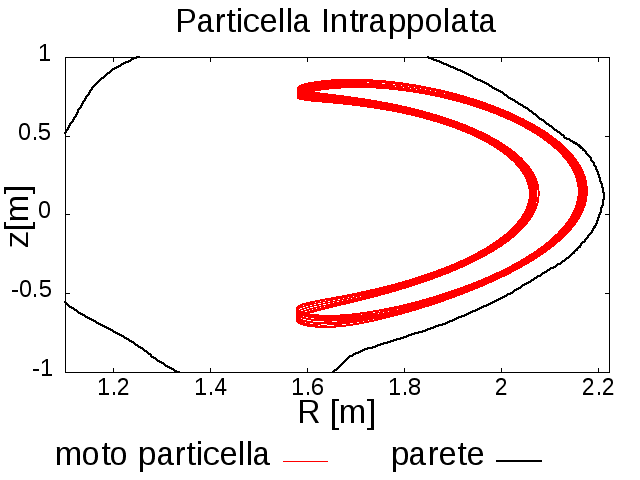
\includegraphics[scale=0.35]{Immagini/Simulazioni/Single/590/2145_E_40k.png}
\end{center}
\begin{center}
Posizione iniziale sul piano mediano, Energia e Pitch-angolo
\end{center}

%{\bfseries Il flusso di particelle sulle pareti potrebbe danneggiare irreparabilmente il dispositivo.}
\end{frame}

% PERDITE 500
\begin{frame}
\frametitle{Scan Energia vs Raggio Iniziale}
\framesubtitle{Equilibrio non Perturbato}
\begin{columns}
	\begin{column}{0.4\textwidth}
		\begin{center}
		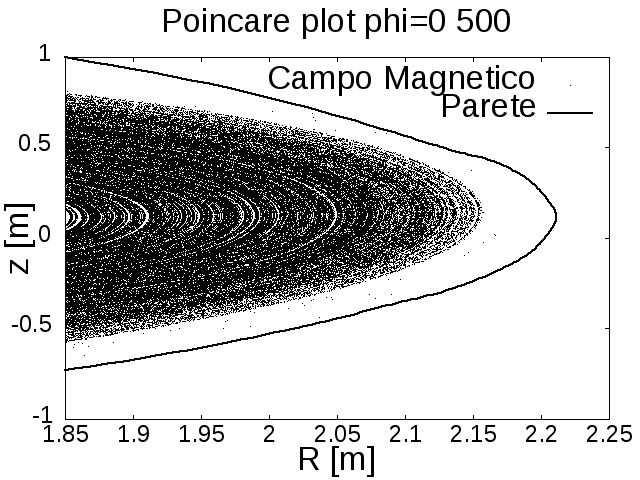
\includegraphics[scale=0.18]{Immagini/Simulazioni/Poincare/poincare_500.png}
		\end{center}
		\begin{center}
		
		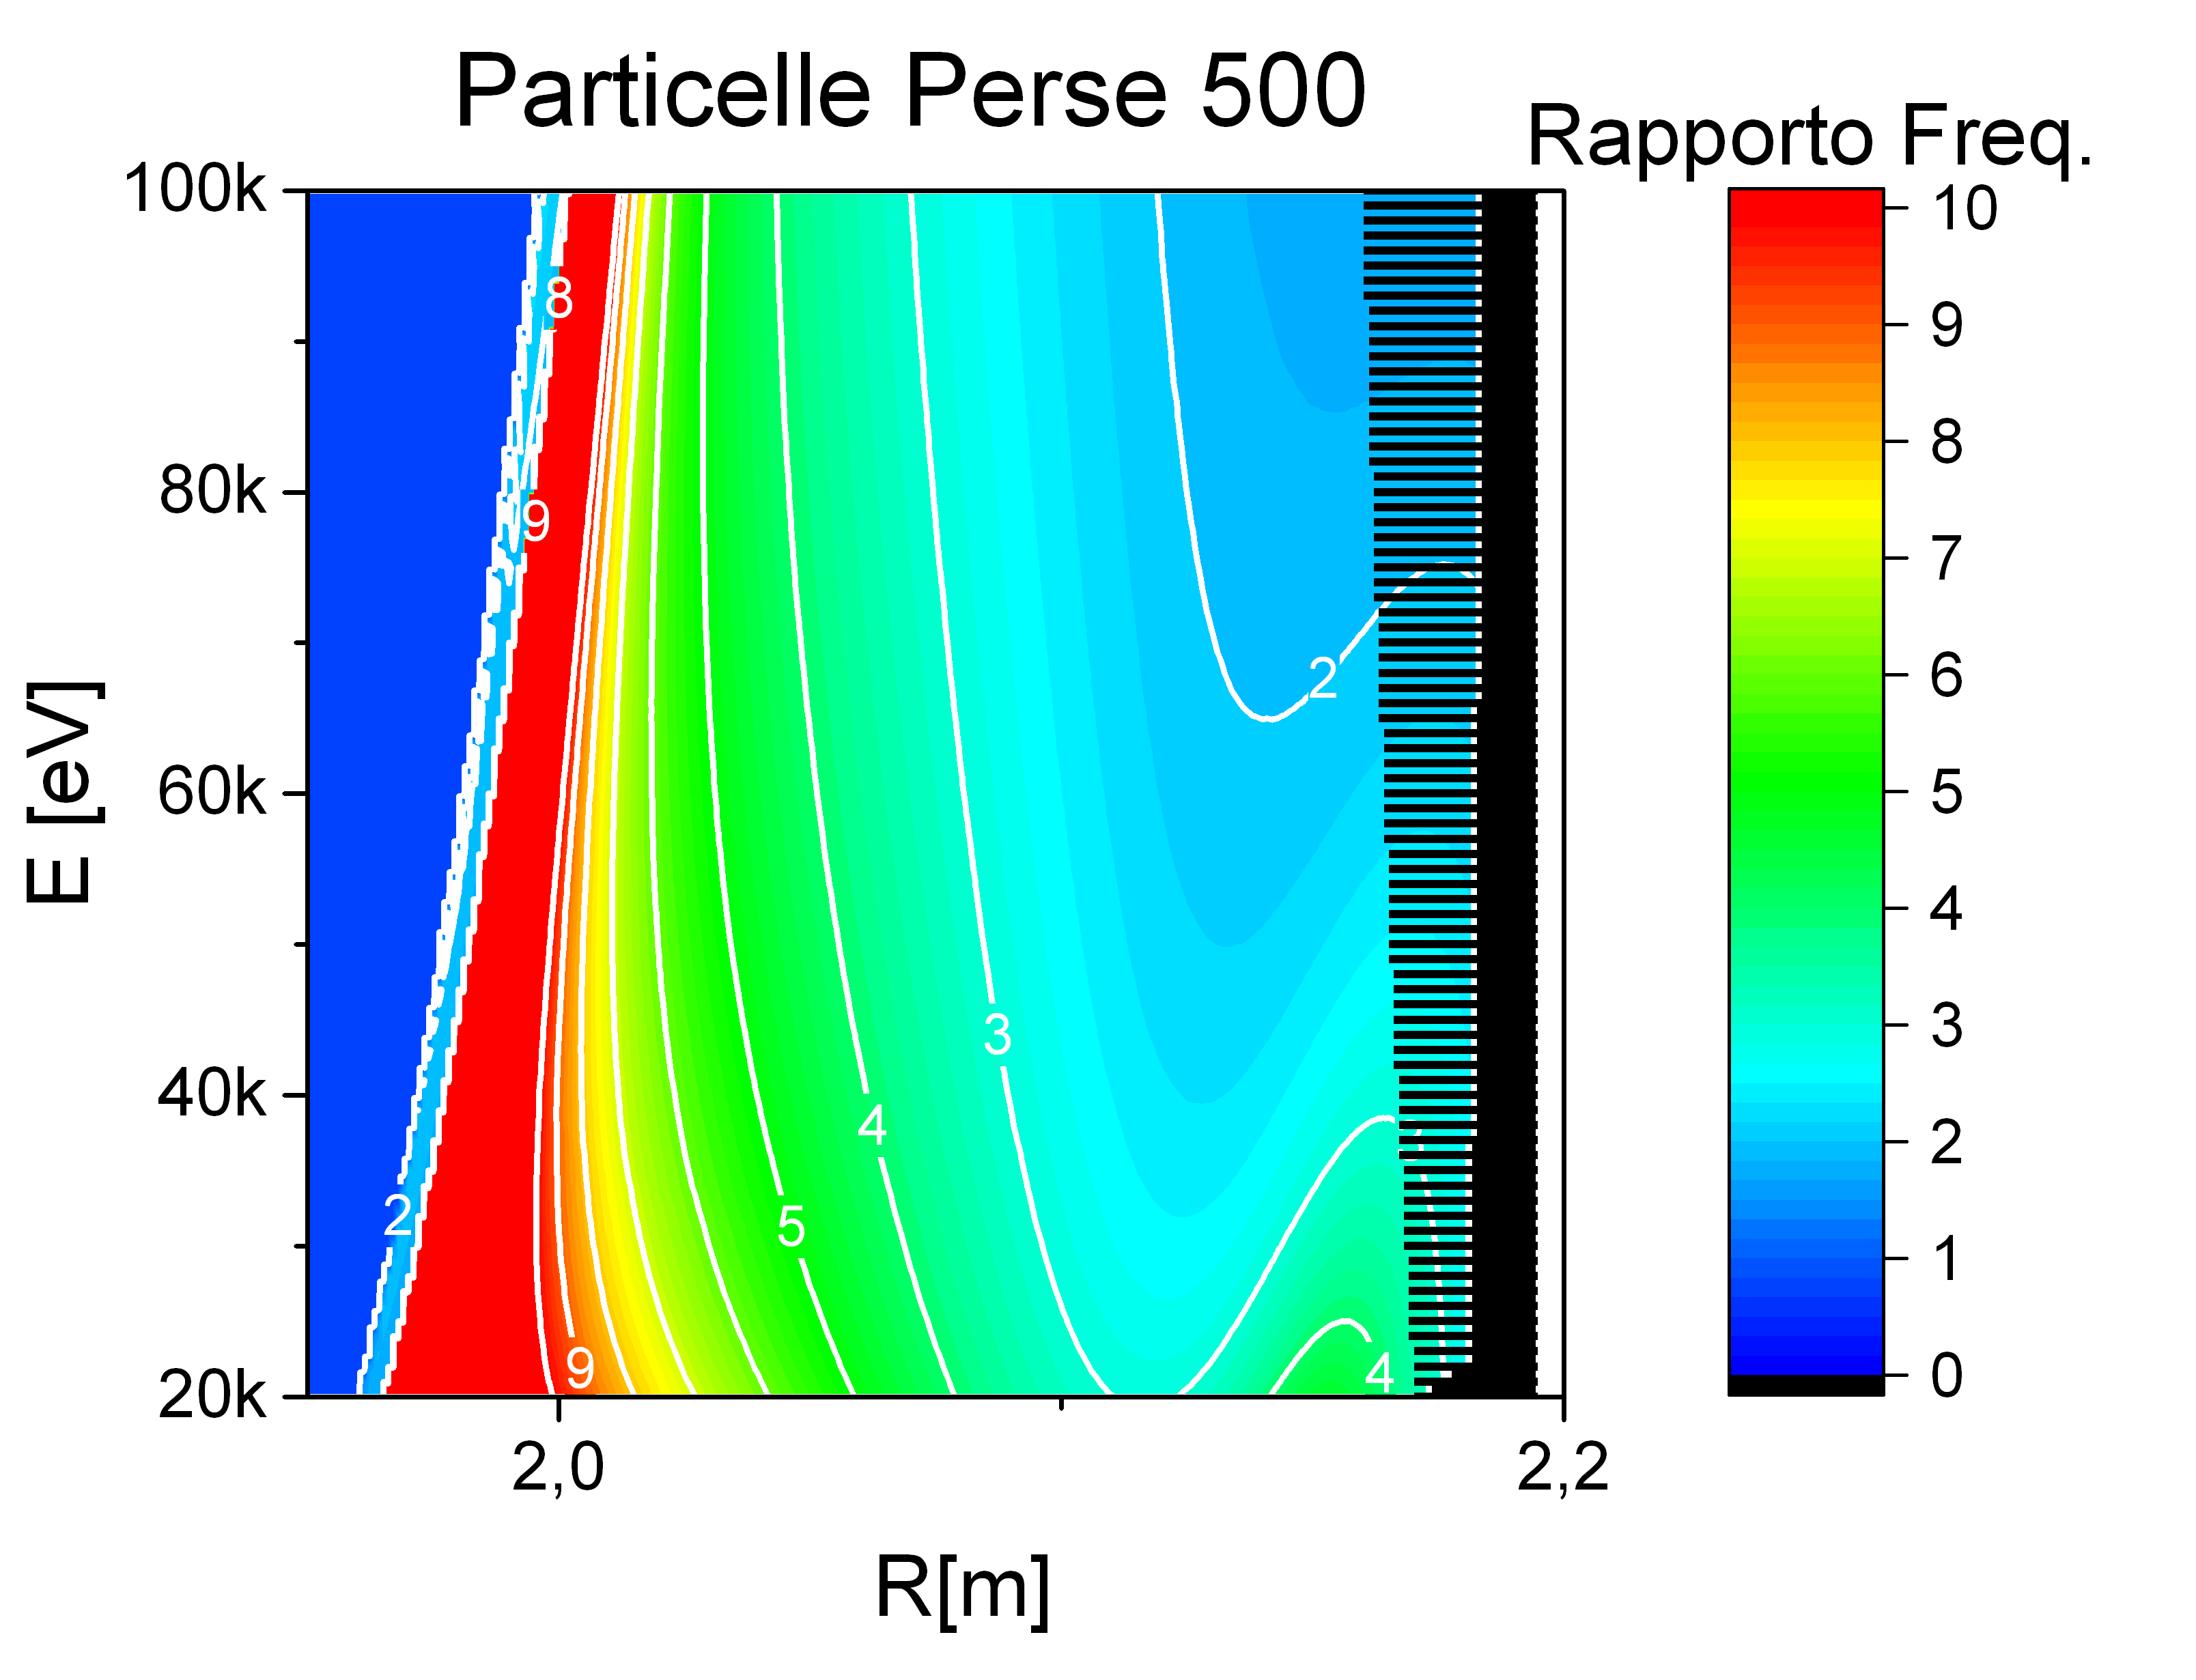
\includegraphics[scale=0.20]{Immagini/Simulazioni/Risonanze/lost_particles_500_160.png}\hspace{-10pt}
		\end{center}
	\end{column}
	\begin{column}{0.4\textwidth}
		\begin{itemize}
			\item Grafico rapporto frequenze caratteristiche
			\item {\bf Punti:} particelle perse con simulazione full orbit
			\item {\bf Regione Nera:} particelle perse con simulazione girocentro
		\end{itemize}
	\end{column}
\end{columns}
\end{frame}

% PERDITE 590
\begin{frame}
\frametitle{Scan Energia vs Raggio Iniziale}
\framesubtitle{Equilibrio Stocastico}
\begin{columns}
	\begin{column}{0.4\textwidth}
		\begin{center}
		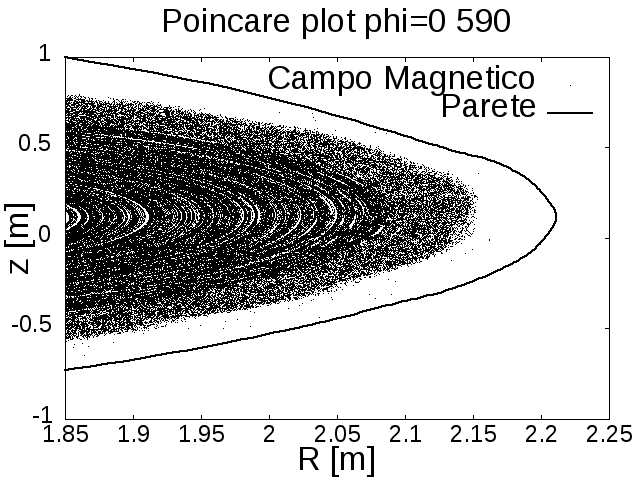
\includegraphics[scale=0.18]{Immagini/Simulazioni/Poincare/poincare_590.png}
		\end{center}
		\begin{center}
		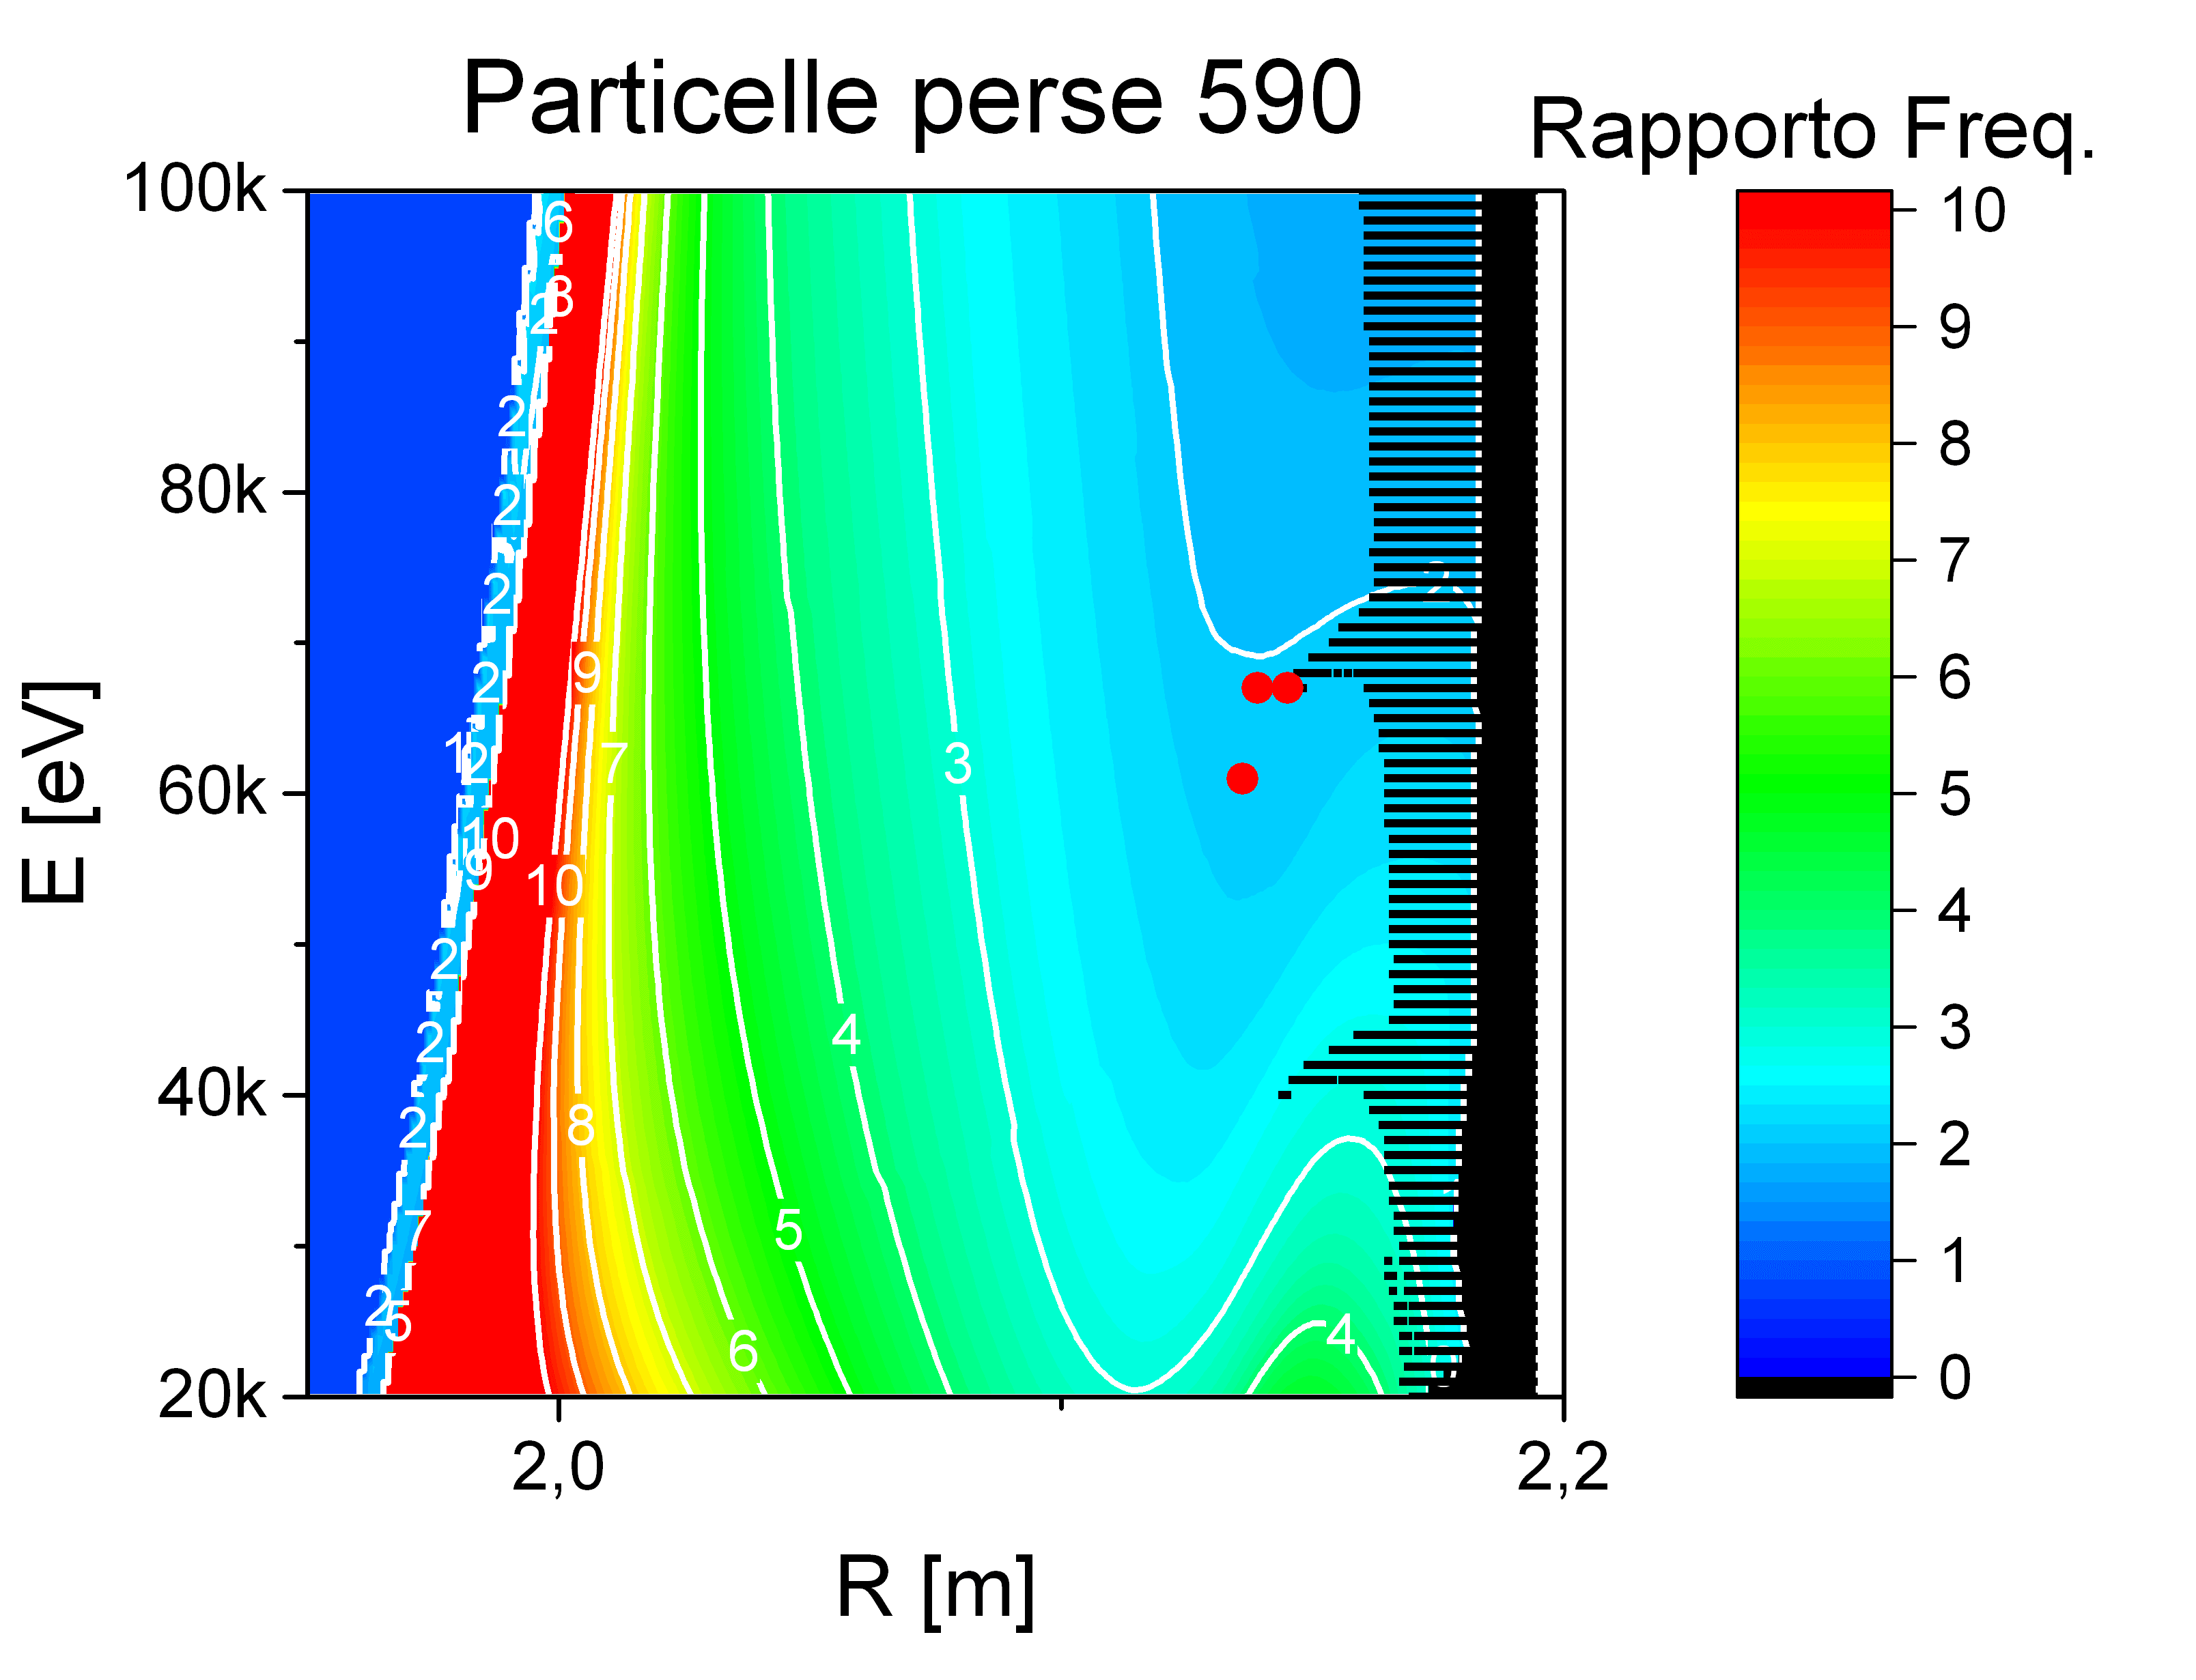
\includegraphics[scale=0.20]{Immagini/Simulazioni/Risonanze/particle_losses_590.png}
		\end{center}
	\end{column}
	\begin{column}{0.4\textwidth}
		\begin{itemize}
			\item Perturbazione curve di livello del rapporto delle frequenze caratteristiche
			\item Aumento dell'area di perdita
			\item Nessuna risonanza geometrica rilevata
			\item Comportamento dipendente da strutture locali
		\end{itemize}
	\end{column}
\end{columns}
\end{frame}

% PERDITE 560
\begin{frame}
\frametitle{Scan Energia vs Raggio Iniziale}
\framesubtitle{Equilibrio "Finger Like"}
\begin{columns}
	\begin{column}{0.4\textwidth}
		\begin{center}
		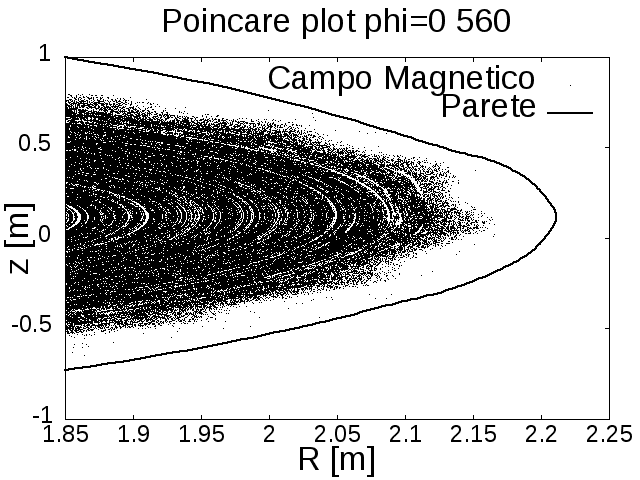
\includegraphics[scale=0.18]{Immagini/Simulazioni/Poincare/poincare_560.png}
		\end{center}
		\begin{center}
		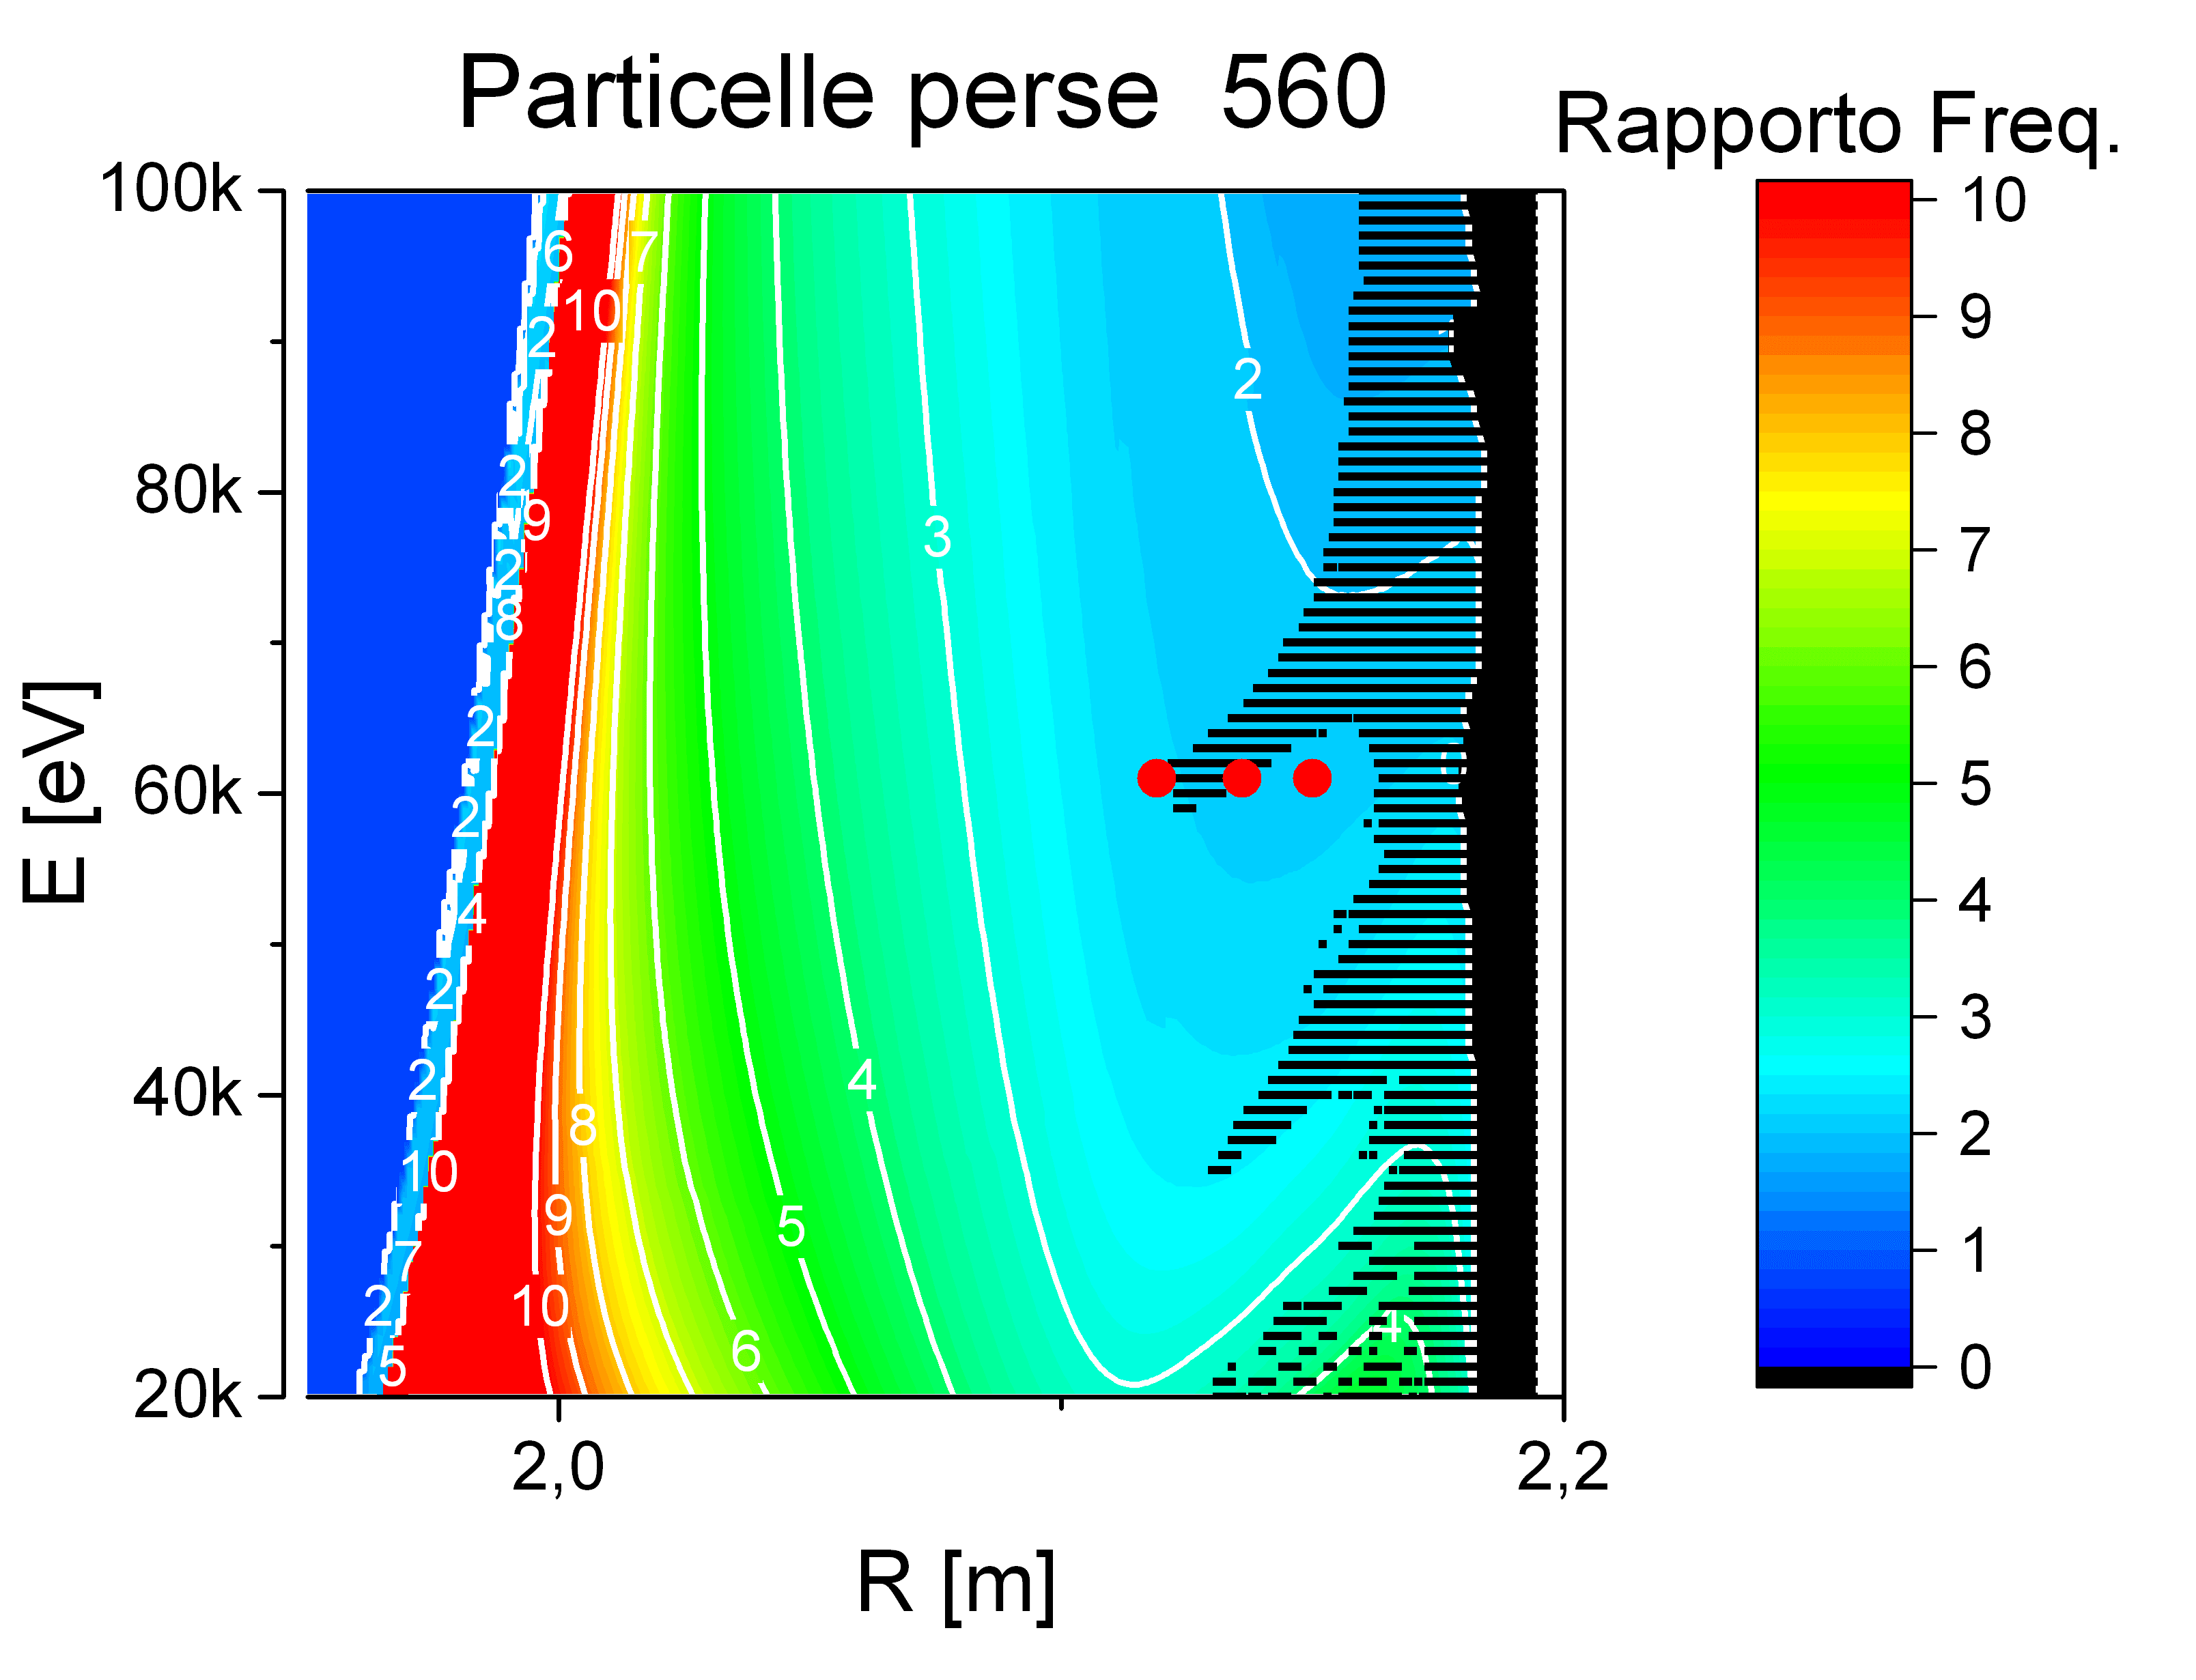
\includegraphics[scale=0.20]{Immagini/Simulazioni/Risonanze/lost_particles.png}
		\end{center}
	\end{column}
	\begin{column}{0.4\textwidth}
		\begin{itemize}
			\item Perturbazione curve di livello del rapporto delle frequenze caratteristiche
			\item Aumento dell'area di perdita
			\item Nessuna risonanza geometrica rilevata
			\item Comportamento dipendente da strutture locali
		\end{itemize}
	\end{column}
\end{columns}
\end{frame}